\subsection{Теорема Фари}

\begin{theorem}[Фари, 1948]
    \label{thm:fari}
    Для всякого планарного графа без кратных ребер и без петель существует укладка, в которой все ребра представлены отрезками.
\end{theorem}

\begin{proof}

    Граф можно предполагать связным.
    
    Рассмотрим произвольную укладку графа, и докажем, что ее можно преобразовать в прямолинейную укладку с сохранением множества граней.
   
    Сперва добавим в граф лишние ребра, чтобы сделать каждую его грань, включая внешнюю, треугольником(триангуляция). После построения укладки эти ребра удалим.
\end{proof}

\begin{lemma}[Лемма о триангуляции]
    Пусть $G$ --- плоский граф без петель, причем в границе каждой грани не менее трех вершин. Тогда существует триангуляция $T$, остовным подграфом которой является $G$.
\end{lemma}

\begin{proof}[ леммы]~

    Пусть $f$ --- грань, граница которой не треугольник.

    Случай 1: граница связна.

    Пусть $V_f$ --- множество вершин грани $f$; $H = G(V_f)$ - индуцированный подграф на $V_f$

    Если граф $H$ неполный, то мы можем добавить в него ребро без образования новых пар кратных ребер; проведем это ребро в грани $f$.

    Пусть $H = K_m$. Так как $|V_f| \geq 3$ и граф $H$ планарен, то $m = 3$ или $4$.

    Если $m = 3$, то граница грани $f$ треугольник.

    Для $m = 4$ разбираем случаи.

    \begin{itemize}
        \item либо граница --- цикл из 4 внешних ребер, и в этом случае невозможно провести оставшиеся два ребра вне грани $f$.
        \item либо граница состоит из треугольников внешних ребер и одного внутреннего, но в этом случае имеем висячую вершину, что невозможно в $K_4$.
    \end{itemize}
    
    \begin{center}
        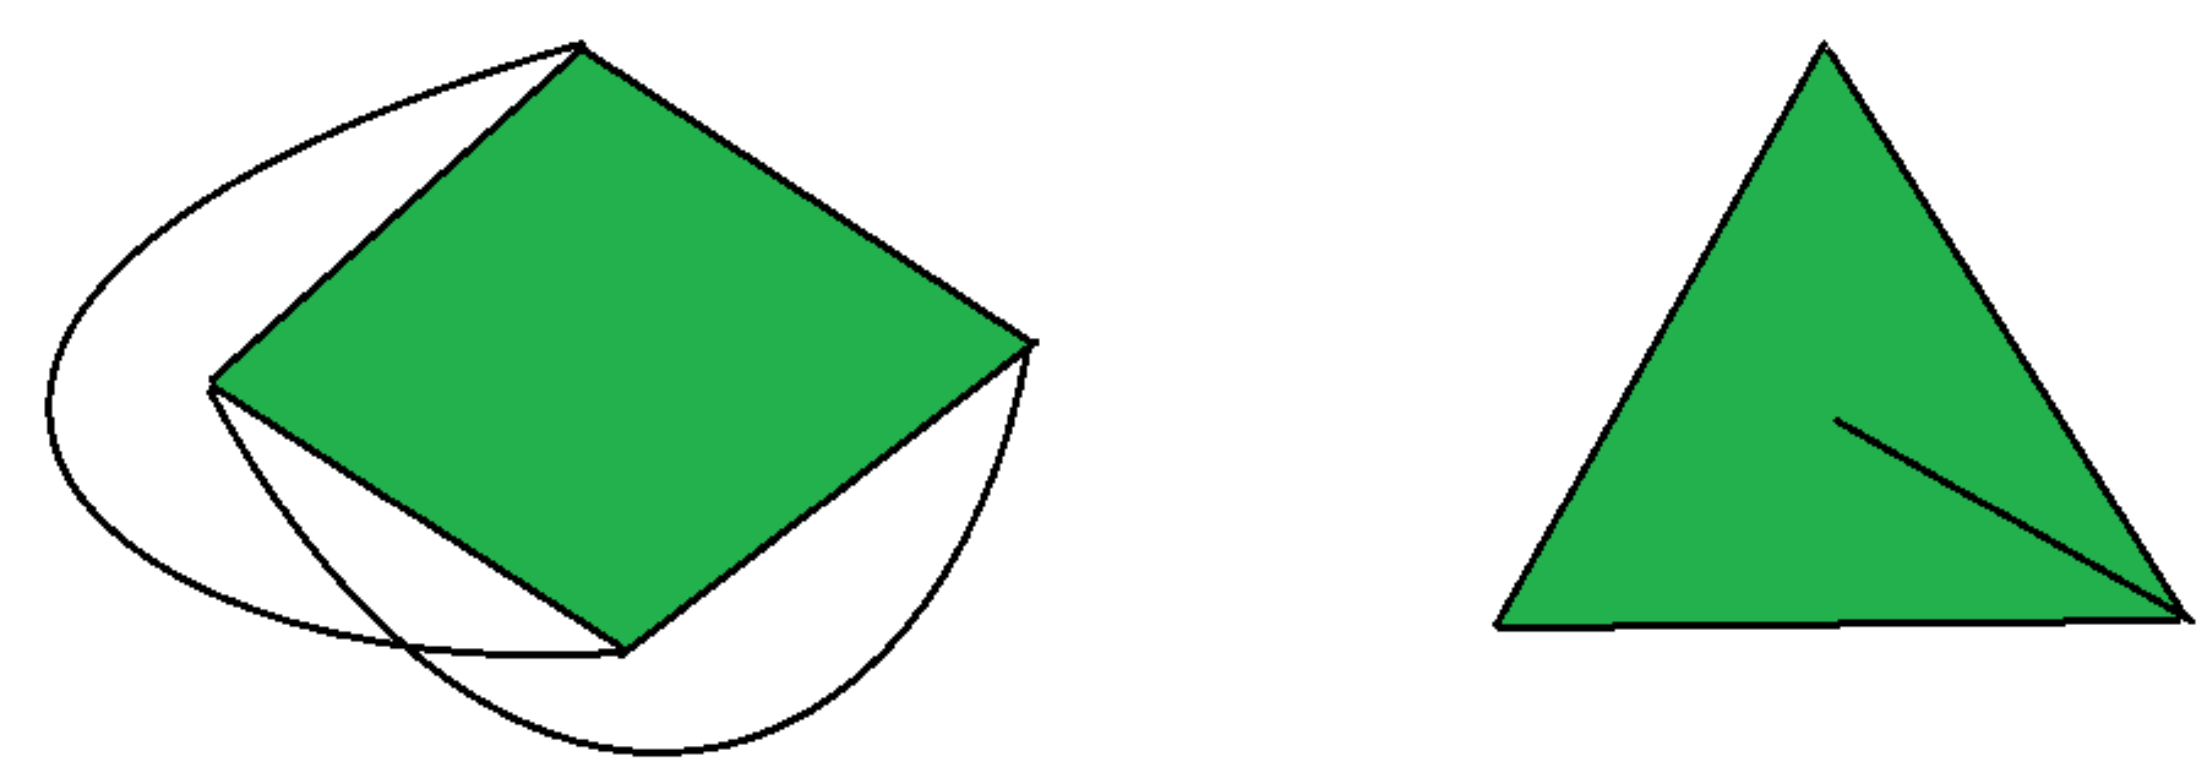
\includegraphics[width=0.5\textwidth]{par30triang.png}
    \end{center}

    Случай 2: граница не связна.

    Пусть $x$ и $y$ --- две вершины из разных компонент связности. Проведем ребро $xy$ внутри грани $f$.

    Это ребро будет внутренним для грани $f$, поэтому длина границы $f$ увеличится на 2. Будем действовать таким образом, пока граница грани не окажется связной.
\end{proof}

\begin{proof}[ теоремы Фари]

    Базис: $|V| = 3$ --- представляется треугольником.

    Шаг индукции: Следствие из \ref*{thm:3v6e} $\implies$ есть вершина $v$: $\deg{v} \leq 5$.

    Докажем, что существует такая вершина, не лежащая на границе внешней грани.

    Пусть в всех вершин не на границе внешней грани $\deg \geq 6$.

    На границе внешней грани ровно три вершины, степень каждой из них не менее чем 2, и должна быть хотя бы одна вершина степени не менее чем 3, потому что иначе весь граф --- треугольник. Тогда
    \[ \sum_{v \in V} \deg v \geq 6(|V| - 3) + 3 + 2 + 2 = 6|V| - 11,\]

    то есть 
    
    \[2|E| \geq 6|V| - 11.\]
    
    Теорема \ref*{thm:3v6e} $\implies 2|E| \leq 6|V| - 12.$ Противоречие.

    Ребра, примыкающие к $v$, принадлежат граням-треугольникам.

    Удаляем $v$, на ее месте остается грань. К этой грани применяем триангуляцию.

    По предположению индукции, для полученного графа есть прямолинейная укладка с сохранением набора граней. 

    Удаляя диагонали, получаем опять большую грань, граница которой --- многоугольник с $\leq 5$ сторонами.
    
    По теореме о художественой галерее всю эту грань может обозревать один сторож. Там, где стоит этот сторож, размещаем вершину $v$; из нее можно провести отрезки во все пять углов. Если сторож стоит в одной из вершин многоугольника, то вершину $v$ можно разместить на небольшом расстоянии от нее.
\end{proof}

\begin{center}
    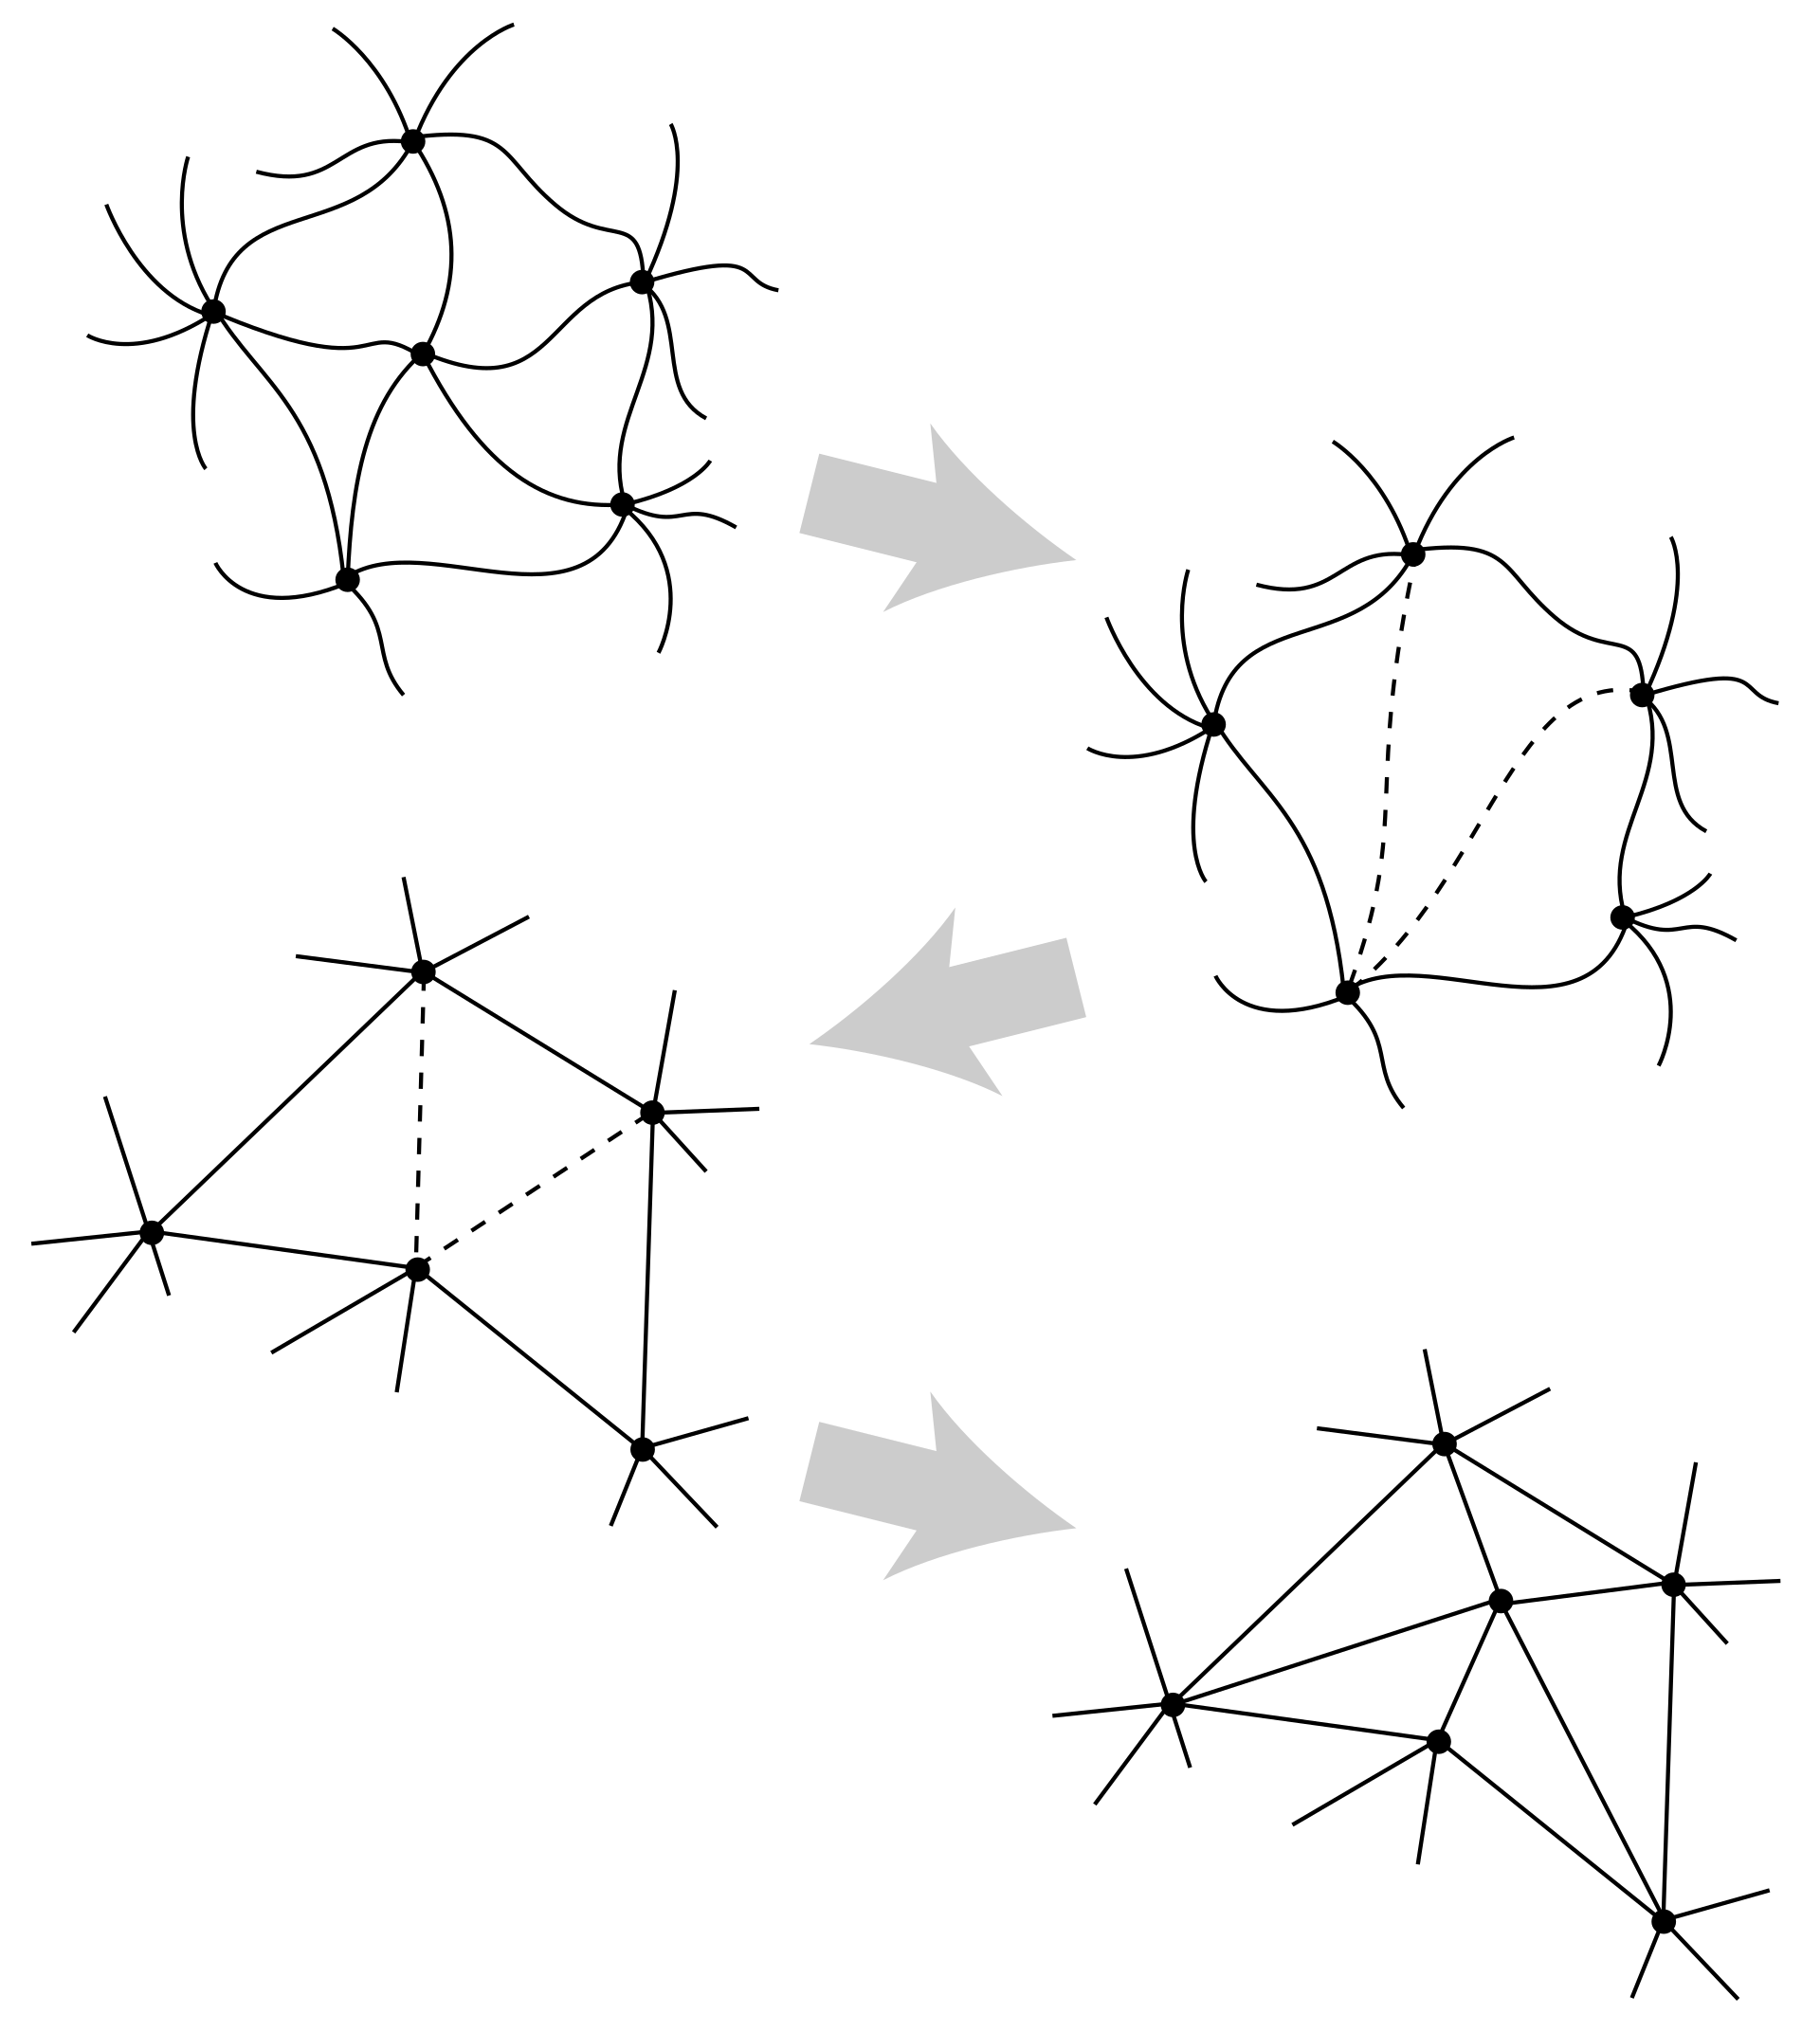
\includegraphics[width=0.5\textwidth]{par30fari.png}
\end{center}